%_____________________________________________________________________________________________ 
% LATEX Template: Department of Comp/IT BTech Project Reports
% Sample Chapter
% Sun Mar 27 10:25:35 IST 2011
%
% Note: Itemization, enumeration and other things not shown. A sample figure is included.
%_____________________________________________________________________________________________ 

\chapter{Introduction}

\section{Importance of Automatic Question Generation (AGS) Systems}

Gauging a student’s knowledge over a certain topic is one of the fundamental
problems in education systems. Quizzing students has long been accepted as one
of the best techniques to solve this problem. Studies conducted over the last
several decades have found that providing students with frequent and good number
of quiz questions leads to better understanding of the topics, than spending an
equal amount of time studying notes or textbooks. Quizzes can be used at several
places in the education domain. They can be used in Massive Open Online Courses (MOOC) to test if a student
has  grasped the concept properly, they can be used as standalone tests in
universities, or they can also be used as practice by students to discern their
command over the subject. 

However, with the volume of information available, generating questions from
domain experts is an expensive and time consuming process. The problem of Automatic
Question Generation (AQG), in the field of Natural Language Processing, aims to
generate questions from a given text, such that students are appropriately
tested on their mastery over the subject.

\section{Neural Networks}

A neural network is an interconnected collections of neurons. The connections
between the neurons are modelled as weights and the final value that the neuron
stores is the weighted summation of all the inputs. A neural network consists of
an input layer, an output layer and multiple hidden layers.

\begin{figure}
	\caption{Basic Neural Network Diagram}
	\centering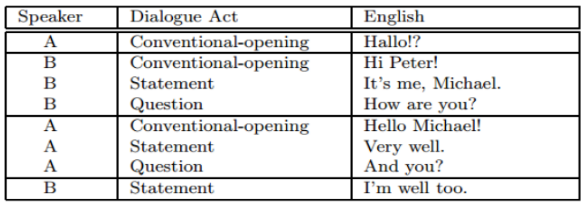
\includegraphics[width=10cm]{1.png}
\end{figure}

\section{Recurrent Neural Networks (RNN)}

Recurrent neural network is a type of artificial neural network. Neural networks had a shortcoming that that they could not remember previous inputs given to the network. This shortcoming was solved by recurrent neural
networks with the help of hidden layers. Because of their internal memory, RNNs
are able to remember important things about the input, which allows them to make
precise predictions of the input that is yet to be processed. Sequential data is an ordered data where
related things follow each other. RNN's have proved extremely useful while working with sequential data. 

\begin{figure}
	\caption{Recurrent vs Feed-forward Neural Network}
	\centering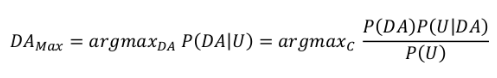
\includegraphics[width=10cm]{2.png}
\end{figure}

Unlike the normal feedforward neural networks, recurrent neural networks feed
the output of previous step to the current step. This helps the network to
memorise the previous inputs. Thus RNN cycles through the information and 
when taking a decision it takes into consideration the current input as
well as whatever it learned from the previous output. As an example, in the
word 'Teacher', by the time a feed forward neural network reaches 'c', it 
has forgotten about the previous inputs 't', 'e' and 'a'. A RNN has the power to remember that. Recurrent Neural
Network adds immediate past to the present. This is important since past data
contains information about what is coming next. 

RNNs apply weight to current and previous input and tweaks their
weights using either the Gradient Descent or Backpropagation Through Time algorithms. Gradient
Descent is an algorithm that is used to iteratively minimize a given function.
Backpropagation Through Time (BPTT) is performing backpropagation on an unrolled RNN. Unrolling is a
visualization and conceptual tool, which helps you to understand what’s going on
within the network. RNN can be viewed as a sequence of Neural Networks that is
trained one after another with backpropagation.

\begin{figure}
	\caption{Structure of a Neuron}
	\centering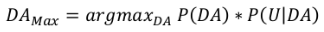
\includegraphics[width=10cm]{3.png}
\end{figure}

The diagram above shows the RNN being unrolled after the equal sign. The
different timesteps are visualized and information gets passed from one timestep
to the next. Within BPTT the error is back-propagated from the last to the first
timestep, while unrolling all the timesteps. This allows calculating the error
for each timestep, which allows updating the weights.

\subsection{Problems with RNN}
Although RNN's are quite powerful because of their inherent ability to remember previous inputs while processing each new one, they have to be used with care as a few of the following problems might occur. 
\begin{enumerate}[align=left]

	\item Training RNNs is a difficult task.

	\item \textbf{Exploding gradient problem :} Exploding gradient is when
		the algorithm assigns an extremely high importance to the weights,
		without much reason. But fortunately, this problem can be easily
		solved by truncating or squashing the gradients.

	\item \textbf{Vanishing gradient problem :} Vanishing gradient is when
		the values of a gradient are too small and the model stops
		learning or takes way too long. This problem is
		solved by the concept of LSTM.

\end{enumerate}

\section{Long Short Term Memory}

Long Short Term Memory (LSTM) is an artificial recurrent neural network.
LSTM can be considered to be an extension to the recurrent neural network, as LSTM has extended memory as compared to RNN. Thus an LSTM is capable of learning things that have very
large time lags between them. The memory used by an LSTM can be attributed to a computer memory as it has functions like read, write or delete information. This is quite different from that of a RNN which uses a vector. 

The memory in LSTM are gated cells. Gated cell means that the cell decides
whether or not to store or delete information based on the importance it assigns
to the information. The assigning of importance takes place through weights which
are learned through the algorithm.

\begin{figure}
	\caption{Structure of a Basic LSTM node}
	\centering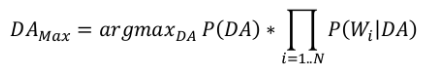
\includegraphics[width=10cm]{4.png}
\end{figure}

A basic LSTM node consists of input gate, output gate and forget gate. The input
gate decides whether or not to let new input in. The forget gate deletes the
information because it is not important. The output gate impacts the output at
the current time step. The gates in a LSTM are analog, in the form of sigmoids,
meaning that they range from 0 to 1. The fact that they are analog, enables them
to do backpropagation with it.

The problem of vanishing gradients which is very common in recurrent neural
networks is solved by LSTM as it keeps the gradient steep enough and therefore
the training short and the accuracy high.
